\documentclass{standalone}
\usepackage{tikz,pgfplots,calc}
\usetikzlibrary{positioning,calc}
\usetikzlibrary{arrows}
\usepackage{tkz-euclide}
\usetkzobj{all}
\renewcommand{\familydefault}{\sfdefault}

\begin{document}
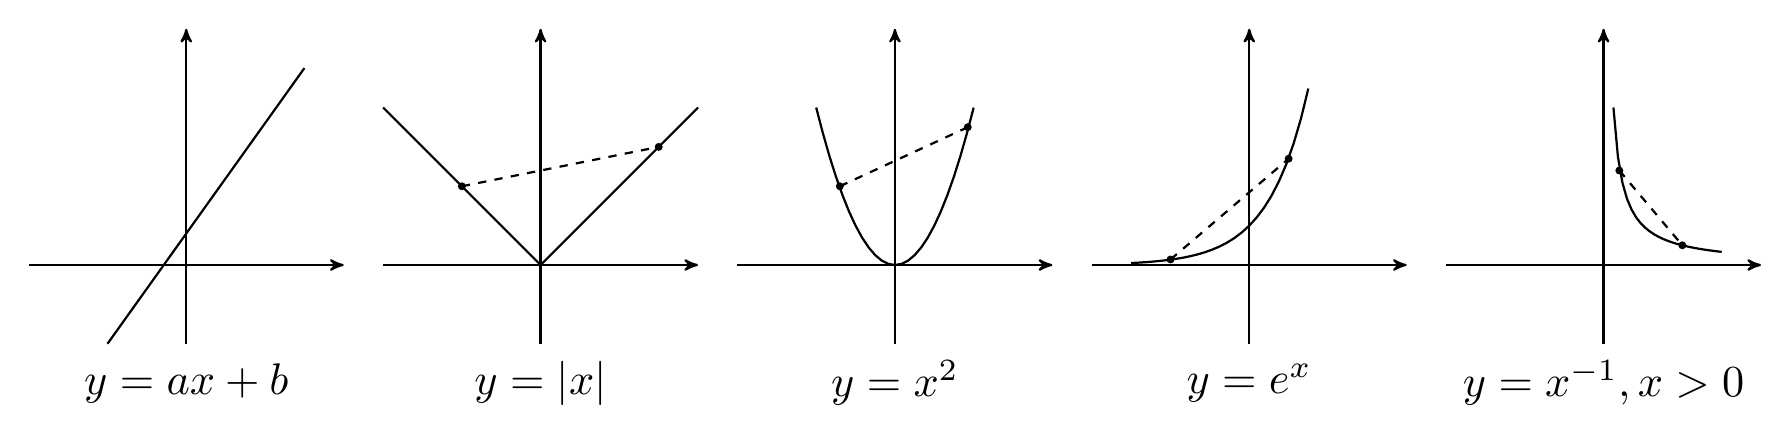
\begin{tikzpicture}[>=stealth', thick]
\def\d{4.5}
\begin{scope}
	\draw [-> ](-2, 0)  --  (2, 0);
	\draw [-> ](0,-1)  --  (0, 3);
	\draw [] (-1, -1)  --  (1.5, 2.5);
	\node [scale = 1.6] at (0, -1.5) {$y = ax + b$};
\end{scope}

\begin{scope}[xshift = 1*\d cm ]
	\draw [-> ](-2, 0)  --  (2, 0);
	\draw [-> ](0,-1)  --  (0, 3);
	\draw [] (-2, 2)  --  (0, 0);
	\draw [] (2, 2)  --  (0, 0);
	\node [scale = 1.6] at (0, -1.5) {$y = |x|$};
	\draw [fill] (-1, 1) circle (1pt);
	\draw [fill] (1.5, 1.5) circle (1pt);
	\draw [dashed] (-1, 1)  --  (1.5, 1.5);
\end{scope}

\begin{scope}[xshift = 2*\d cm ]
	\draw [-> ](-2, 0)  --  (2, 0);
	\draw [-> ](0,-1)  --  (0, 3);
	\draw[scale=0.5,domain=-2:2,variable=\x,] plot ({\x},{\x*\x});
	\node [scale = 1.6] at (0, -1.5) {$y = x^2$};

	\draw [fill] (-.7, 1) circle (1pt);
	\draw [fill] (.925, 1.75) circle (1pt);
	\draw [dashed] (-.7, 1)  --  (.925, 1.75);

\end{scope}


\begin{scope}[xshift = 3*\d cm ]
	\draw [-> ](-2, 0)  --  (2, 0);
	\draw [-> ](0,-1)  --  (0, 3);
	\draw[scale=0.5,domain=-3:1.5,variable=\x,] plot ({\x},{exp(\x)});
	\node [scale = 1.6] at (0, -1.5) {$y = e^x$};

	\draw [fill] (-1, .07) circle (1pt);
	\draw [fill] (.5, 1.35) circle (1pt);
	\draw [dashed] (-1, .07)  --  (.5, 1.35);
\end{scope}

\begin{scope}[xshift = 4*\d cm ]
	\draw [-> ](-2, 0)  --  (2, 0);
	\draw [-> ](0,-1)  --  (0, 3);
	\draw[scale=0.5,domain=.25:3,variable=\x,] plot ({\x},{\x^-1});
	\node [scale = 1.6] at (0, -1.5) {$y = x^{-1}, x > 0$};

	\draw [fill] (.2, 1.2) circle (1pt);
	\draw [fill] (1, .25) circle (1pt);
	% \draw [fill] (.5, 1.35) circle (1pt);
	\draw [dashed] (.2, 1.2)  --  (1, .25);

\end{scope}

\end{tikzpicture}
\end{document}